% ThreatTron research manuscript
% Overleaf: upload this file only; references.bib is generated by filecontents.
% Replace the author block and the three placeholder figures before submission.
\begin{filecontents*}{references.bib}
@techreport{nist80061, author={Cichonski, Paul and Millar, Tom and Grance, Tim and Scarfone, Karen}, title={Computer Security Incident Handling Guide}, institution={NIST}, number={SP 800-61 Rev. 2}, year={2012}, doi={10.6028/NIST.SP.800-61r2}}
@techreport{nist80092, author={Kent, Karen and Souppaya, Murugiah}, title={Guide to Computer Security Log Management}, institution={NIST}, number={SP 800-92}, year={2006}, doi={10.6028/NIST.SP.800-92}}
@techreport{nist80053, author={Joint Task Force}, title={Security and Privacy Controls for Information Systems and Organizations}, institution={NIST}, number={SP 800-53 Rev. 5}, year={2020}, doi={10.6028/NIST.SP.800-53r5}}
@inproceedings{sommer2010, author={Sommer, Robin and Paxson, Vern}, title={Outside the Closed World: On Using Machine Learning for Network Intrusion Detection}, booktitle={2010 IEEE Symposium on Security and Privacy}, pages={305--316}, year={2010}, doi={10.1109/SP.2010.25}}
@article{chandola2009, author={Chandola, Varun and Banerjee, Arindam and Kumar, Vipin}, title={Anomaly Detection: A Survey}, journal={ACM Computing Surveys}, volume={41}, number={3}, pages={1--58}, year={2009}, doi={10.1145/1541880.1541882}}
@article{greitzer2010, author={Greitzer, Frank L. and others}, title={Combining Traditional Cyber Security Audit Data with Psychosocial Data: A Bayesian Approach to Identifying Suspected Insiders}, journal={Insider Threats in Cyber Security}, pages={127--140}, year={2010}, doi={10.1007/978-1-4419-7133-3_7}}
@article{breiman2001, author={Breiman, Leo}, title={Random Forests}, journal={Machine Learning}, volume={45}, number={1}, pages={5--32}, year={2001}, doi={10.1023/A:1010933404324}}
@article{ke2017, author={Ke, Guolin and others}, title={LightGBM: A Highly Efficient Gradient Boosting Decision Tree}, journal={Advances in Neural Information Processing Systems}, volume={30}, year={2017}}
@article{lundberg2017, author={Lundberg, Scott M. and Lee, Su-In}, title={A Unified Approach to Interpreting Model Predictions}, journal={Advances in Neural Information Processing Systems}, volume={30}, year={2017}}
@article{pedregosa2011, author={Pedregosa, Fabian and others}, title={Scikit-learn: Machine Learning in Python}, journal={Journal of Machine Learning Research}, volume={12}, pages={2825--2830}, year={2011}}
@misc{psutil, author={Rodola, Giampaolo}, title={psutil: Cross-platform Process and System Utilities}, year={2024}, howpublished={\url{https://github.com/giampaolo/psutil}}}
@misc{cert, author={{Carnegie Mellon University Software Engineering Institute}}, title={CERT Insider Threat Test Dataset}, year={2016}, howpublished={\url{https://www.sei.cmu.edu/our-work/cybersecurity/insider-threat/}}}
@misc{mitreattack, author={{MITRE}}, title={MITRE ATT\&CK Enterprise}, year={2024}, howpublished={\url{https://attack.mitre.org/}}}
@article{saltzer1975, author={Saltzer, Jerome H. and Schroeder, Michael D.}, title={The Protection of Information in Computer Systems}, journal={Proceedings of the IEEE}, volume={63}, number={9}, pages={1278--1308}, year={1975}, doi={10.1109/PROC.1975.9939}}
\end{filecontents*}

\documentclass[conference]{IEEEtran}
\usepackage{cite}
\usepackage{amsmath,amssymb}
\usepackage{booktabs}
\usepackage{array}
\usepackage{multirow}
\usepackage{graphicx}
\usepackage{xcolor}
\usepackage{url}
\usepackage{hyperref}
\usepackage{tikz}
\usetikzlibrary{arrows.meta,positioning,fit,shapes.geometric}
\hypersetup{colorlinks=true,linkcolor=blue,citecolor=blue,urlcolor=blue}
\newcommand{\placeholder}[1]{\fbox{\begin{minipage}[c][#1][c]{0.92\columnwidth}\centering\footnotesize\textit{Insert the corresponding project export or screenshot here.}\end{minipage}}}

\title{ThreatTron: A Privacy-Aware, Explainable and Multimodal Architecture for\\Host-Based Insider-Threat Detection}
\author{\IEEEauthorblockN{Author Name}\IEEEauthorblockA{Department, University or Organization\\City, Country\\email@example.com}}

\begin{document}
\maketitle

\begin{abstract}
Insider-threat detection requires a broad behavioral view because no single event type reliably distinguishes ordinary work from preparation for data misuse. This paper presents ThreatTron, a host-centered security architecture that combines endpoint telemetry, behaviorally engineered features, a supervised ensemble, an unsupervised anomaly model, explainable risk scores, and an analyst-facing investigation workflow. The architecture is privacy-aware: it separates collection domains, hashes network endpoint identifiers before storage, avoids network-payload inspection, and supports bounded retention. We evaluate the reproducible artifacts currently present in the project rather than reporting fabricated production results. The pipeline processes 1,000 users through 35 engineered features and combines LightGBM, Random Forest, logistic regression, and Isolation Forest scores with configuration weights of 0.5, 0.2, 0.1, and 0.2. In the saved prediction output, 61 users exceed the operational risk threshold of 0.8; the accompanying observable-validation report records 61 captured insiders among 191 labeled insiders and 130 not captured under its stricter matching protocol. The explanation output gives three leading features per user; total file activity is the most frequent first-ranked feature for 448 users. These measurements demonstrate an auditable research platform and a practical high-confidence triage workflow. They also define the next experiments required for publication-grade generalization, calibration, and cross-environment validation.
\end{abstract}
\begin{IEEEkeywords}
insider-threat detection, endpoint detection and response, behavioral analytics, privacy-aware telemetry, ensemble learning, explainable AI
\end{IEEEkeywords}

\section{Introduction}
Modern organizations generate security evidence across logons, email, web activity, file operations, removable devices, processes, system state, and network connections. The same breadth that improves visibility creates a difficult research problem: a useful detector must integrate heterogeneous event streams without turning every unusual action into an accusation. Insider-threat programs are especially sensitive because the subject may be an authorized employee, a compromised account, or a benign user whose work is atypical. Detection therefore requires context, careful data governance, and an analyst who can challenge model output.

ThreatTron is a research prototype for this problem. Its data-collection agents produce structured endpoint events; a backend stores sessions, events, assessments, alerts, and investigation notes; and a behavioral-model pipeline transforms user-level activity into engineered features. The model layer uses a complementary ensemble: LightGBM and Random Forest capture nonlinear interactions, logistic regression supplies a comparatively transparent linear signal, and Isolation Forest provides an unsupervised deviation score. A weighted risk score and local feature explanations connect prediction to triage.

This paper treats the project as a system contribution rather than as a claim that a prototype replaces a security operations center. The central research question is: can a privacy-aware, multimodal endpoint architecture convert diverse user activity into an explainable risk-ranking signal that is useful for analyst triage while limiting unnecessary collection?

The contributions are:
\begin{enumerate}
\item an end-to-end architecture joining collection, session provenance, feature engineering, ensemble inference, explanation, alerting, and investigation;
\item a data-minimization design for network telemetry that stores connection metadata and salted endpoint digests rather than packet payloads;
\item a reproducible description of the current 1,000-user, 35-feature experiment and its saved outputs; and
\item a publication-ready evaluation protocol that distinguishes model-label performance from stricter observable-ground-truth validation.
\end{enumerate}

\section{Research Context}
\subsection{Insider Threats as Behavioral Inference}
An insider event is not defined by one field such as an unusual port or a large file count. It is inferred from a combination of timing, sequence, access context, and deviation from a user's or peer group's baseline. The CERT Insider Threat Test Dataset is widely used to study synthetic insider scenarios and provides a useful experimental reference, but no benchmark is a perfect substitute for an organization's telemetry and policy context \cite{cert}. ThreatTron therefore aggregates multiple domains into user-level features before classification.

\subsection{Anomaly Detection and Operational Risk}
Anomaly detection methods identify observations that differ from an expected distribution \cite{chandola2009}. In security, this is attractive because novel attacks may not have labels; however, rarity is not equivalent to malice. Machine learning also fails when training and deployment environments differ, when feedback is delayed, or when analysts cannot interpret a score \cite{sommer2010}. ThreatTron's risk score is consequently designed for ranking and investigation, not automatic punishment or account termination.

\subsection{Explainability and Security Governance}
Feature attribution can help an analyst understand why an alert was ranked highly. SHAP formalizes additive feature contributions for a range of models \cite{lundberg2017}, but an explanation is not a causal proof. NIST guidance emphasizes controlled collection, access protection, retention, and incident-handling procedures \cite{nist80061,nist80092,nist80053}. These requirements motivate the project's session identifiers, evidence references, role-aware backend workflow, and explicit separation between raw collection and derived assessments.

\section{System Goals and Threat Model}
\subsection{Goals}
The system has five goals: (G1) collect complementary endpoint evidence; (G2) produce a stable user-level risk ranking; (G3) show the evidence and leading features behind a ranking; (G4) preserve event provenance for investigation; and (G5) minimize the sensitivity of collected network data. A sixth practical goal is deployability: collection should run as an agent and remain useful even when the dashboard or model service is temporarily unavailable.

\subsection{Adversary Model}
We consider an external attacker who compromises an endpoint, an insider who abuses authorized access, and a compromised account that performs activity inconsistent with its historical pattern. We also consider an attacker who reads an event store. We do not assume the operating system, Python runtime, or administrator account is trustworthy after full host compromise. Accordingly, hashing protects persisted endpoint identifiers from casual disclosure but does not defeat a malicious process that reads values before transformation or obtains the salt.

\subsection{Non-goals and Safety Boundaries}
ThreatTron is not a packet-content inspection system, a malware sandbox, or a proof of user intent. It should not be used for covert surveillance, employment decisions without human review, or automatic punitive action. The deployment must have authorization, a documented purpose, least-privilege access, and a deletion policy. These boundaries are part of the system's research validity because a detector that violates its data-governance assumptions is not a safe operational contribution.

\section{Architecture}
Figure~\ref{fig:architecture} summarizes the data path. Agents create a session, collect domain-specific events, and send structured batches. The backend persists events by session and agent identity. Feature engineering aggregates events into user-level vectors. The model pipeline trains or loads four complementary estimators, normalizes their scores, and produces a weighted risk score. The alert and investigation layers preserve the link from a score to evidence references and analyst feedback.

\begin{figure*}[t]
\centering
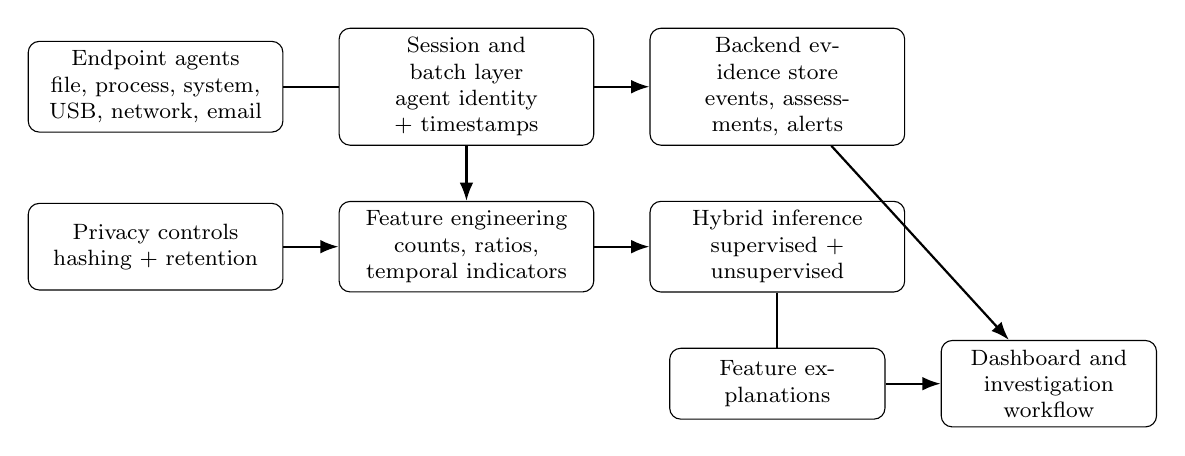
\begin{tikzpicture}[node distance=7mm and 7mm, box/.style={draw,rounded corners,align=center,minimum height=11mm,text width=3.0cm,font=\footnotesize}, small/.style={draw,rounded corners,align=center,minimum height=9mm,text width=2.5cm,font=\footnotesize}, arrow/.style={-{Latex},thick}]
\node[box] (agents) {Endpoint agents\\file, process, system, USB, network, email};
\node[box,right=of agents] (session) {Session and batch layer\\agent identity + timestamps};
\node[box,right=of session] (backend) {Backend evidence store\\events, assessments, alerts};
\node[box,below=of session] (features) {Feature engineering\\counts, ratios, temporal indicators};
\node[box,right=of features] (models) {Hybrid inference\\supervised + unsupervised};
\node[box,left=of features] (privacy) {Privacy controls\\hashing + retention};
\node[small,below=of models] (explain) {Feature explanations};
\node[small,right=of explain] (analyst) {Dashboard and\\investigation workflow};
\draw[arrow] (agents)--(session)--(backend);
\draw[arrow] (session)--(features);
\draw[arrow] (privacy)--(features);
\draw[arrow] (features)--(models);
\draw[arrow] (models)--(explain)--(analyst);
\draw[arrow] (backend)--(analyst);
\end{tikzpicture}
\caption{ThreatTron architecture. Collection is separated from model inference, while session identifiers and evidence references preserve provenance across the pipeline.}
\label{fig:architecture}
\end{figure*}

\subsection{Multimodal Endpoint Collection}
The repository contains collectors for file activity, process activity, system resources, USB events, network connections, and email-related signals. This separation is valuable because domains have different privacy and failure characteristics. A file event may contain a path; a network event needs only connection metadata; a process event may provide parent-child context; and a system event provides load context. The common session identifier makes these records joinable without requiring one monolithic collector.

\subsection{Network Data Minimization}
For network observations, the agent records timestamp, local and remote ports, socket status, optional process identity, and salted SHA-256 digests of endpoint addresses. Let $H_s(x)=\operatorname{SHA256}(s\Vert x)$, where $s$ is an installation-specific secret. The digest enables grouping repeated observations within one installation while preventing the raw address from being written to the database. Payload bytes are outside the schema. This follows the principle of collecting the minimum information necessary for a stated detection task, while acknowledging that timestamps, ports, process names, and repeated digests remain potentially sensitive.

\subsection{Backend Evidence and Investigation}
The backend data model separates agent sessions from domain events and from derived objects such as risk assessments, alerts, investigations, and notes. This distinction allows a new model to be evaluated without rewriting the original evidence and permits an analyst to mark an alert's status or false-positive feedback without deleting the supporting event. The design is aligned with evidence-preservation practices, but production deployment still requires authentication, authorization, encryption in transit, encrypted backups, and audit logging.

\section{Feature Construction}
The behavioral pipeline merges user-level records and creates derived ratios and intensity measures. The current preprocessed artifact contains 1,000 rows and 35 columns, including identifiers and engineered behavioral features. Representative base measures include total logons, after-hours logons, weekend logons, failed logons, total emails, emails with attachments, external emails, total HTTP activity, suspicious HTTP activity, total file operations, executable or archive files, after-hours file operations, device count, and distinct computers. Derived features include ratios such as attachment ratio, suspicious-file ratio, suspicious-HTTP ratio, and an exfiltration-intensity measure.

For a user $u$, the feature vector is $\mathbf{x}_u=[x_{u1},\ldots,x_{ud}]$, where $d=35$ in the saved artifact. Count features preserve activity volume, while normalized ratios reduce the effect of different observation durations. Temporal features retain potentially important context without storing message content. Missing and malformed values are handled in preprocessing; the exact transformation, imputation, and scaling configuration should be versioned with each experiment.

\begin{table}[t]
\caption{Feature families represented in the current 35-column artifact}
\label{tab:features}
\centering
\footnotesize
\begin{tabular}{p{0.28\columnwidth}p{0.60\columnwidth}}
\toprule
Family & Examples and detection purpose \\
\midrule
Authentication & total, after-hours, weekend, failed logons; unusual access timing \\
Email & total, external, attachment counts; staging or exfiltration context \\
Web & total and suspicious HTTP; uncommon destinations or browsing patterns \\
Files & total, executable/archive, after-hours operations; collection and staging signals \\
Devices & device count and removable-media activity; transfer context \\
Host context & distinct computers and derived ratios; peer and baseline comparison \\
\bottomrule
\end{tabular}
\end{table}

\section{Hybrid Risk Model}
\subsection{Complementary Estimators}
The supervised component contains LightGBM, Random Forest, and logistic regression. Gradient-boosted trees are effective for nonlinear interactions in tabular data \cite{ke2017}; Random Forest aggregates randomized trees and is robust to heterogeneous feature scales \cite{breiman2001}; logistic regression provides a lower-complexity reference model. Isolation Forest supplies an unsupervised anomaly signal for deviations that may not be represented by the labeled examples \cite{chandola2009}.

Each model produces a score that is normalized to $[0,1]$ using the training-pass parameters. If $s_L$, $s_R$, $s_G$, and $s_A$ denote normalized LightGBM, Random Forest, logistic, and anomaly scores, the current configuration defines
\begin{equation}
 R(u)=0.5s_L(u)+0.2s_R(u)+0.1s_G(u)+0.2s_A(u).
\label{eq:risk}
\end{equation}
An operational alert is generated when $R(u)>0.8$. The weights and threshold are configuration parameters, not universal constants; they must be tuned and calibrated on a development split and then frozen for test evaluation.

\subsection{Explainability Layer}
The pipeline writes three leading features for every user. This compact explanation answers which behavioral dimensions deserve inspection before the analyst opens supporting events. A production report should additionally include signed contribution values, the model version, feature timestamp range, and a counterfactual or baseline comparison. The current top-feature output is still useful as an auditable bridge between a score and the data-generating behavior.

\section{Experimental Setup and Data Provenance}
This section reports only values present in the repository artifacts. The experiment uses the saved behavioral-model version 0.3 outputs. The merged, engineered, and preprocessed CSV artifacts each contain 1,000 user rows; the engineered and preprocessed artifacts contain 35 columns. The prediction file contains one row per user with four normalized component scores, a final risk score, and a binary label. The explanation file contains one row per user and three ranked feature names. The validation report states that 1,000 users were examined and uses a strict observable comparison with 191 insider labels.

The distinction between these artifacts matters. The prediction CSV's label column is a model-pipeline output, whereas the observable-validation report compares risk alerts with a separate ground-truth procedure. They should not be silently merged into one metric. We therefore report both views and label them explicitly.

\begin{table}[t]
\caption{Reproducible artifact inventory and measured counts}
\label{tab:inventory}
\centering
\footnotesize
\begin{tabular}{p{0.43\columnwidth}r p{0.25\columnwidth}}
\toprule
Artifact or setting & Value & Source \\
\midrule
Users in merged/preprocessed data & 1,000 & CSV row count \\
Columns in engineered data & 35 & CSV header \\
Normalized model components & 4 & prediction header \\
Risk-score threshold & 0.8 & config.yaml \\
Risk weights (LGBM/RF/logistic/anomaly) & 0.5/0.2/0.1/0.2 & config.yaml \\
Users above threshold & 61 & validation report \\
Observable insiders & 191 & validation report \\
Captured under observable protocol & 61 & validation report \\
Top features per explanation & 3 & explanations.csv \\
\bottomrule
\end{tabular}
\end{table}

\section{Implementation and Deployment Model}
\subsection{Collection Lifecycle}
An endpoint starts a collection session with an agent identifier, hostname, and start time. Domain collectors then produce events with a common session identifier. Batching reduces request overhead and gives the backend an atomic unit for validation. The sender should retry transient failures with bounded backoff and must not duplicate events when a request is retried; an event identifier or idempotency key is therefore recommended for production. A local queue can preserve evidence during a short network outage, but its size and lifetime should be bounded by the retention policy.

The Windows-oriented collector is intended to run as a background service. Service packaging is a deployment concern rather than a detection feature: a release asset should pin dependencies, record the model and schema versions, and provide a clear uninstall path. Startup failure, permission denial, clock skew, and unavailable backend connectivity should be surfaced as health events, not silently interpreted as absence of suspicious behavior. A lightweight health endpoint or heartbeat allows an administrator to distinguish ``no activity'' from ``no collector.''

\subsection{Backend and API Boundaries}
The backend presents separate routes for domain events and security workflow objects. This separation permits a front end to request aggregated views without receiving every raw event. API responses should enforce the caller's organization, campus, agent, and role scope before filtering records. Pagination, time-window filters, and server-side aggregation are required when event volume grows. A model service should accept a versioned feature schema and return the model version, score, threshold, and evidence references together; otherwise an analyst cannot reliably reproduce an alert shown in the interface.

\subsection{Operational State and Failure Semantics}
The system has four useful states: collecting, queued, analyzed, and under investigation. A session can be collecting while its events are queued; an alert can be analyzed while its associated evidence remains immutable; and an investigation can be closed while feedback is retained for later calibration. These states are preferable to treating a Boolean ``threat'' flag as the entire operational truth. They also support audit questions such as who changed an alert, which model version produced it, and whether the evidence was available at decision time.

\subsection{Comparison with Alternative Designs}
A packet-capture sensor offers richer content but increases storage and privacy exposure and often lacks process attribution on the originating host. A single supervised classifier is simple to operate but is brittle when labels are incomplete or a new behavior is absent from training data. A purely unsupervised detector can surface novelty but may rank routine workload differences as threats. ThreatTron's contribution is a middle path: endpoint metadata and process context are combined with multiple statistical views, while an analyst remains in the loop. The comparison is qualitative in this paper; a future experiment should measure detection and resource costs under identical workloads.

\begin{table}[t]
\caption{Design choices compared with common alternatives}
\label{tab:designcompare}
\centering
\footnotesize
\begin{tabular}{p{0.22\columnwidth}p{0.22\columnwidth}p{0.43\columnwidth}}
\toprule
Design & Primary strength & Trade-off addressed by ThreatTron \\
\midrule
Packet capture & Content-rich evidence & Higher privacy, storage, and governance burden \\
Single supervised model & Simple scoring & Weakness under unseen or shifted behavior \\
Pure anomaly detection & Finds novelty without labels & Benign rarity can create alert fatigue \\
Manual log review & Human context & Does not scale across event volume \\
ThreatTron & Multimodal, ranked, explainable evidence & Requires calibration and disciplined review \\
\bottomrule
\end{tabular}
\end{table}

\section{Ablation and Sensitivity Plan}
The current weighted score demonstrates an architecture, but a publishable claim about the ensemble requires ablations. First, compare each component alone with the weighted score under the same split. Second, remove one telemetry family at a time (authentication, email, web, file, device, and host context) and measure the change in precision--recall AUC and alert volume. Third, perturb the polling interval and retention window for the endpoint agent. Fourth, compare the fixed threshold of 0.8 with thresholds selected on a development set under a specified analyst alert budget.

Sensitivity analysis should report how many users cross the threshold when each weight changes by a small amount. For example, let $\Delta_w$ be a perturbation of one ensemble weight followed by renormalization. Report the Jaccard similarity between the original and perturbed alert sets, along with the change in captured-insider rate. A stable alert set is easier to operate and audit; a highly unstable set indicates that calibration or uncertainty reporting is needed.

The experiment should also test temporal leakage. Randomly splitting rows can place nearly identical observations from one user in both training and test sets, producing over-optimistic results. User-disjoint and time-ordered splits answer different questions and should be reported separately. The CERT dataset and related insider-threat studies are useful for controlled comparison, but the strongest evidence will come from a documented holdout period that was not used to select features, weights, or thresholds.

\section{Threat-to-Evidence Mapping}
The feature families can be connected to investigation hypotheses without claiming a one-to-one mapping from behavior to intent. A burst of after-hours logons may motivate a review of authentication and device context. Large file activity combined with executable or archive operations may motivate a staging hypothesis. Attachment and external-email ratios may motivate a transfer review. Suspicious web activity may motivate destination and process correlation. Device activity may explain why file operations increased. The value of multimodality is that these hypotheses can be tested against multiple sessions rather than inferred from one isolated count.

\begin{table}[t]
\caption{Illustrative analyst hypotheses and corroborating evidence}
\label{tab:hypotheses}
\centering
\footnotesize
\begin{tabular}{p{0.29\columnwidth}p{0.55\columnwidth}}
\toprule
Risk signal & Evidence to review before disposition \\
\midrule
After-hours logon burst & authentication timing, host, preceding failures, peer schedule \\
File and archive spike & file paths, process parent, device activity, time sequence \\
Attachment or external-email ratio & sender domain, attachment metadata, destination policy \\
Suspicious web ratio & process identity, destination category, concurrent file actions \\
New device context & USB event, user authorization, files accessed after mount \\
High anomaly score alone & baseline window, workload change, model explanation, corroboration \\
\bottomrule
\end{tabular}
\end{table}

This mapping is deliberately phrased as a review aid rather than a rule engine. A security analyst can reject a hypothesis when policy or business context explains the observation. The investigation note should record both supporting and contradictory evidence, which makes later model review more informative than a binary label alone.

\section{Results}
\subsection{Risk-Score Distribution and Alert Volume}
Independent inspection of the saved prediction CSV gives 1,000 rows. The final risk score has minimum 0.00034, maximum 0.90494, mean 0.10757, and median 0.04059. At the configured threshold of 0.8, 61 rows are above threshold. The largest scores are 0.90494, 0.89909, 0.88674, 0.88139, and 0.87500, demonstrating that the score ranks a small high-risk tail rather than assigning uniformly high risk.

\begin{table}[t]
\caption{Descriptive statistics from the saved prediction output ($n=1000$)}
\label{tab:scorestats}
\centering
\footnotesize
\begin{tabular}{lrrrr}
\toprule
Score & Minimum & Median & Mean & Maximum \\
\midrule
LightGBM normalized & 0.0000 & $8.8\times10^{-9}$ & 0.0700 & 1.0000 \\
Random Forest normalized & 0.0000 & 0.0000 & 0.0788 & 1.0000 \\
Logistic normalized & 0.0000 & 0.0025 & 0.1298 & 1.0000 \\
Anomaly normalized & 0.0000 & 0.1756 & 0.2192 & 1.0000 \\
Final risk score & 0.00034 & 0.0406 & 0.1076 & 0.9049 \\
\bottomrule
\end{tabular}
\end{table}

The component statistics show why the ensemble is useful as a research design. The anomaly component has a higher median than the supervised components, while the final score remains dominated by the LightGBM weight. Thus the ensemble can combine a broad novelty signal with more selective supervised evidence without treating either source as sufficient by itself.

\subsection{Observable Validation}
The saved validation report examines 1,000 users, flags 61 users above 0.8, and reports 61 true insiders captured out of 191 observable insiders. This is a capture rate of $61/191=31.9\%$. Under the report's matching definition, the 61 flagged users correspond to the 61 captured users, implying zero reported false positives in that alert set. This should be read as a high-confidence alert-set result for the stated protocol, not as a general precision estimate for every deployment. The report also lists 130 insiders not captured, which motivates threshold calibration, richer temporal modeling, and evaluation on additional environments.

\begin{table}[t]
\caption{Observable-validation summary reported by the project}
\label{tab:validation}
\centering
\footnotesize
\begin{tabular}{lr}
\toprule
Measure & Value \\
\midrule
Users examined & 1,000 \\
Risk threshold & $>$0.8 \\
Users flagged & 61 \\
Observable insiders & 191 \\
Captured insiders & 61 \\
Not captured & 130 \\
Captured-insider rate & 31.9\% \\
Reported alert-set false positives & 0 \\
\bottomrule
\end{tabular}
\end{table}

\subsection{Explanation Coverage}
The explanation artifact contains 1,000 rows, each with three feature names. The most frequent first-ranked feature is \texttt{total\_file}, appearing for 448 users (44.8\%). It is followed by \texttt{total\_device} for 260 users (26.0\%), \texttt{after\_hours\_logons} for 102 users (10.2\%), and \texttt{overall\_suspicious\_ratio} for 99 users (9.9\%). These counts do not prove that file activity causes risk; they identify which feature families dominate the current explanation output and therefore which evidence should be inspected for data quality and policy relevance.

\begin{table}[t]
\caption{Most frequent first-ranked explanation features}
\label{tab:explanations}
\centering
\footnotesize
\begin{tabular}{lrr}
\toprule
Feature & Users & Share \\
\midrule
\texttt{total\_file} & 448 & 44.8\% \\
\texttt{total\_device} & 260 & 26.0\% \\
\texttt{after\_hours\_logons} & 102 & 10.2\% \\
\texttt{overall\_suspicious\_ratio} & 99 & 9.9\% \\
\texttt{total\_logons} & 43 & 4.3\% \\
\texttt{attachment\_ratio} & 36 & 3.6\% \\
Other features & 12 & 1.2\% \\
\bottomrule
\end{tabular}
\end{table}

\section{Analyst Workflow and Human Factors}
Figure~\ref{fig:workflow} presents the intended analyst loop. A risk score is only the entry point. The analyst checks the contributing features, opens the associated time range and event evidence, compares activity with policy and peer context, and records a disposition. Feedback should be used for monitoring and future calibration, not for silently relabeling historical ground truth. This workflow reduces the risk that a high score is mistaken for intent.

\begin{figure}[t]
\centering
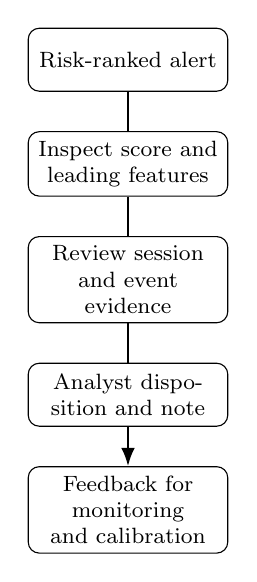
\begin{tikzpicture}[node distance=5mm, n/.style={draw,rounded corners,align=center,text width=2.3cm,minimum height=8mm,font=\footnotesize}, a/.style={-{Latex},thick}]
\node[n] (alert) {Risk-ranked alert};
\node[n,below=of alert] (why) {Inspect score and leading features};
\node[n,below=of why] (evidence) {Review session and event evidence};
\node[n,below=of evidence] (decide) {Analyst disposition and note};
\node[n,below=of decide] (feedback) {Feedback for monitoring and calibration};
\draw[a] (alert)--(why)--(evidence)--(decide)--(feedback);
\end{tikzpicture}
\caption{Human-in-the-loop triage workflow. A model score initiates review; it does not determine intent or sanction.}
\label{fig:workflow}
\end{figure}

\section{Security and Privacy Analysis}
\subsection{Data Minimization}
The network collector excludes payload contents and hashes endpoint identifiers before persistence. This reduces direct exposure of addresses and communications, but it does not make the data anonymous. Repeated hashes remain linkable, and ports, process names, file paths, timestamps, and aggregate counts can reveal sensitive behavior. Salt rotation can reduce long-term linkability at the cost of longitudinal correlation.

\subsection{Access Control and Provenance}
A secure deployment should use separate service identities for collection, inference, and investigation; enforce role-based access; encrypt transport and backups; and record access to event evidence. Session identifiers and evidence references provide a foundation for provenance, while the backend's alert and investigation objects provide a place to record review outcomes. These controls should be verified with negative authorization tests before any real deployment.

\subsection{Adversarial Considerations}
An attacker may evade polling by creating short-lived connections, mimic ordinary activity, poison a baseline, or deliberately generate noisy events. A compromised endpoint may tamper with local collection. Defense-in-depth therefore includes authenticated agents, integrity-protected batches, clock validation, server-side rate limits, and independent network or identity telemetry. The project's design supports correlation but does not claim complete observability.

\section{Reproducibility Protocol}
To reproduce the reported counts, preserve the commit identifier, configuration file, Python and package versions, input-data provenance, and output hashes. Run preprocessing, training, prediction, explanation, and observable validation as separate recorded stages. Split data by user and time where possible to prevent leakage between nearly identical records. Save the trained estimators, normalizers, feature schema, threshold, and weights with the experiment.

For a stronger publication study, create three partitions: a development partition for feature and threshold selection, a test partition for a single final report, and a temporal holdout representing future behavior. Repeat with multiple seeds and report confidence intervals. Evaluate precision, recall, F1, precision--recall AUC, false-positive rate, calibration error, alert volume per 1,000 users, and time-to-triage. Include ablations for each model family and each telemetry domain so that the value of multimodality is measurable rather than assumed.

\begin{figure}[t]
\centering
\placeholder{3.0cm}
\caption{Suggested results figure: precision--recall curves for LightGBM, Random Forest, logistic regression, Isolation Forest, and the weighted ensemble on a held-out split. Include bootstrap confidence bands.}
\label{fig:pr}
\end{figure}

\section{Limitations and Future Research}
The present artifacts establish a functioning research pipeline and provide concrete measurements, but they do not by themselves establish cross-organization generalization. The observable-validation report and prediction labels represent different evaluation views and should remain separate. The current explanation file stores feature names rather than full signed attributions. The network component is metadata-only by design, so content-dependent threats require other controls. A polling collector may miss brief connections, and endpoint compromise can invalidate local evidence. These are research boundaries, not reasons to discard the architecture.

Future work should (1) add temporal sequence features and per-user baselines; (2) calibrate scores using a development set; (3) evaluate domain ablations and cost-sensitive thresholds; (4) add signed explanations and evidence timelines; (5) test salt rotation and linkage leakage; (6) measure resource overhead under continuous Windows service operation; (7) evaluate multi-organization isolation with explicit tenant and campus scopes; and (8) conduct a blinded analyst study measuring triage accuracy and time. These experiments would turn the current platform into a stronger empirical conference contribution.

\section{Conclusion}
ThreatTron demonstrates a practical way to connect privacy-aware endpoint collection, multimodal behavioral features, hybrid machine learning, explainability, and analyst workflow. The current artifacts contain 1,000 users, 35 engineered columns, four normalized model components, 61 threshold-level alerts, and 1,000 three-feature explanations. The saved observable validation captures 61 of 191 labeled insiders under its strict protocol, while the explanation output identifies file activity as the leading first-ranked feature for 448 users. These are concrete, inspectable results that support a research narrative centered on auditable triage rather than inflated claims. With controlled temporal evaluation, calibration, ablations, and secure deployment testing, the architecture provides a credible foundation for privacy-aware insider-threat research.

\section*{Acknowledgment}
The authors should add dataset acknowledgments, institutional review or ethics approval information, and funding statements here where applicable. Do not include private user data, credentials, or unreleased endpoint identifiers in the paper or its supplementary material.

\bibliographystyle{IEEEtran}
\bibliography{references}
\end{document}
